
\pagestyle{headings}
Zu Beginn des vierten Tages sollte die Messstruktur nun um die dritte Art der Demodulation, der Multiplikation mit dem Träger, erweitert werden.
Dieser neue Case ist in Abb. \ref{fig:messstruktur_dam_case3} dargestellt.
\begin{figure}[H]
	\centering
	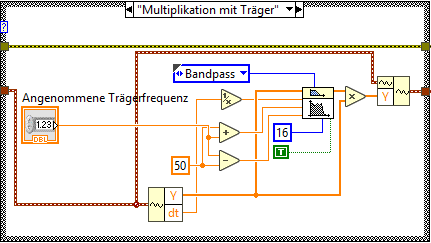
\includegraphics[width=\textwidth]{pic/messstruktur_dam_case3.png}
	\caption{Case für den Fall der  Multiplikation mit dem Träger als Demodulationsart.}
	\label{fig:messstruktur_dam_case3}	
\end{figure} 
In diesem Falle muss eine geschätzte Trägerfrequenz angegeben werden, da diese nicht einfach dem eingehenden Signal zu extrahieren ist.
Zudem muss, um das Auftreten ungewollter Seitenbänder zu unterdrücken, das Trägersignal vorher mit einem Bandpass so verändert werden, dass die Trägerfrequenz möglichst die einzige verbliebene Frequenz in dem Signal ist, sodass dann bei der Multiplikation mit dem moduliertem Signal die Trägerfrequenz wegfällt und nur die Frequenzen des Ursprungssignals $S(t)$ überbleibt.
Vollständig verschwindet die Trägerfrequenz so jedoch nicht, da auch Frequenzanteile mit doppelter Trägerfrequenz auftreten.
Diese lassen sich aber wie zuvor durch den Tiefpass hinter dem Case filtern.
Um sich gleichzeitig auch noch um den Gleichanteil, zu kümmern wird dieser Tiefpass hinter dem Case durch einen Bandpass ersetzt, was in Abb. \ref{fig:messstruktur_dafpm} in der vollständigen Messstruktur zu sehen ist.
	
\

Bevor es jedoch zu Vervollständigung der Messstruktur durch Erweiterung der Demodulation von frequenz- und phasenmodulierten Signalen kommt, war die nächste Aufgabe zunächst einmal das Modulations-VI um die beiden fehlenden Arten der Modulation zu erweitern.
An dieser Stelle ließ sich dann auch der Fehler in der Verkabelung feststellen und die Soundkarte konnte nun die Position des Funktionsgenerators ersetzen.
Dabei wurde der Audio-Ausgang des Rechners mit dem ADC dort verbunden, wo vorher der Funktionsgenerator angeschlossen war.
	
\

Die Erweiterung des Modulations-VI um Frequenz- und Phasenmodulation belief sich auf die in Abb. \ref{fig:am} nicht dargestellten Cases.
Diese sind in der Abbildung \ref{fig:fmpm} dargestellt.
Für diese wurden folgende Formeln herangezogen und in LabVIEW modelliert:
\begin{align}
	\label{eq:FM} S_\text{FM}(t) &= \cos{(2\pi[f_\text{T}t + k \cdot \int_{-\infty}^{t}{S(\tau)\dd{\tau}}])} \\
	\label{eq:PM} S_\text{PM}(t) &= \cos{(2\pi[f_\text{T}t + k \cdot S(t)])}.
\end{align} 
Wie auch bei dem Abspeichern wird eine for-Schleife verwendet um die Zeit $t_i$ über den Kehrwert der Messfrequenz in $i$ Schritten zu konstruieren.
Der Modulationsgrad $m$ aus der Amplitudenmodulation entspricht hier dem $k$ aus der Formel.
Im Wesentlichen unterscheiden sich der Fall der Frequenzmodulation von der Phasenmodulation nur dadurch, dass das zu modulierende Signal vor weiteren Rechenoperationen noch integriert wird.
Da die Amplitude für das ausgehende Signal für den Modulationsprozess hier keine große Rolle spielt, solange sie ungleich null ist, wird diese hier auf eins gesetzt.
Durch einfache Rechenoperationen wird das Argument des Kosinus aufgestellt und dann in die Funktion gegeben.
		
\
	
Jeweils ein Beispiel des Frontpanels für die beiden neuen Modulationsverfahren ist in Abb. \ref{fig:fm_example} (Frequenzmodulation) bzw. Abb. \ref{fig:pm_example} (Phasenmodulation) dargestellt.
Auffällig ist die charakteristische Menge der auftretenden Seitenbänder verglichen mit der Amplitudenmodulation.
Auch hierfür sind weitere Beispiele im Anhang (Abschnitt \ref{sec:anhang}) vorzufinden.

\begin{figure}[H]
	\centering
	\begin{subfigure}[c]{\textwidth}
		\centering
		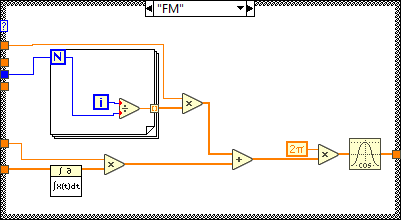
\includegraphics[width=0.9\textwidth]{pic/fm.png}
		\subcaption{Case für die Berechnung eines frequenzmodulierten Signals.}
	\end{subfigure}
	\begin{subfigure}[c]{\textwidth}
		\centering
		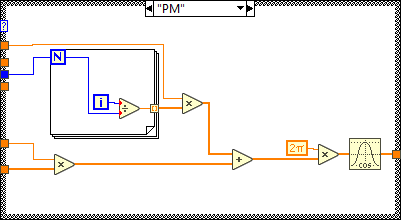
\includegraphics[width=0.9\textwidth]{pic/pm.png}
		\subcaption{Case für die Berechnung eines phasenmodulierten Signals.}
	\end{subfigure}	
	\caption{Alternative Fälle für den Case für die Modulationsart in Abb. \ref{fig:am}.}
	\label{fig:fmpm}	
\end{figure}

\newpage
\pagestyle{empty}
\begin{figure}[H]
	\centering
	\begin{subfigure}[c]{\textwidth}
		\centering
		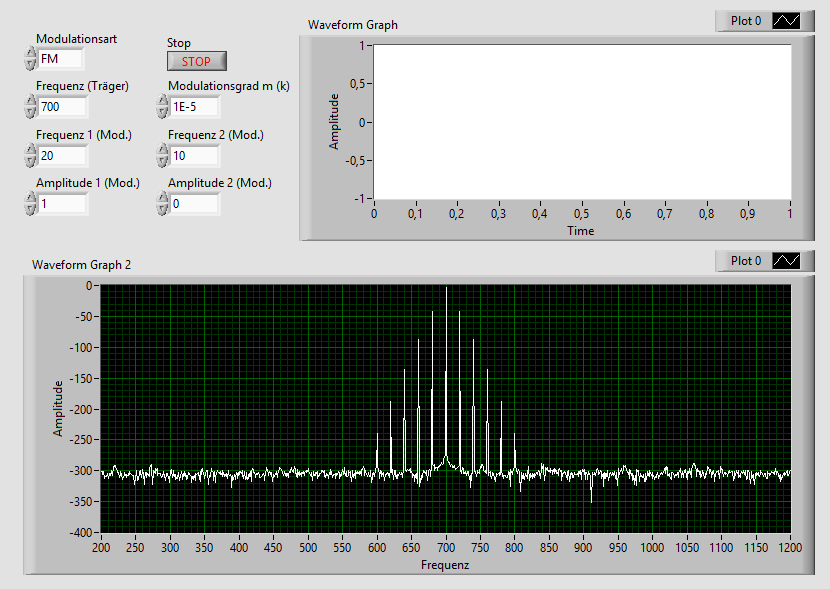
\includegraphics[width=0.9\textwidth]{pic/fm_example.png}
		\caption{Frequenzmodulation}
		\label{fig:fm_example}	
	\end{subfigure}
	\vspace{0.5cm}
	\begin{subfigure}[c]{\textwidth}
		\centering
		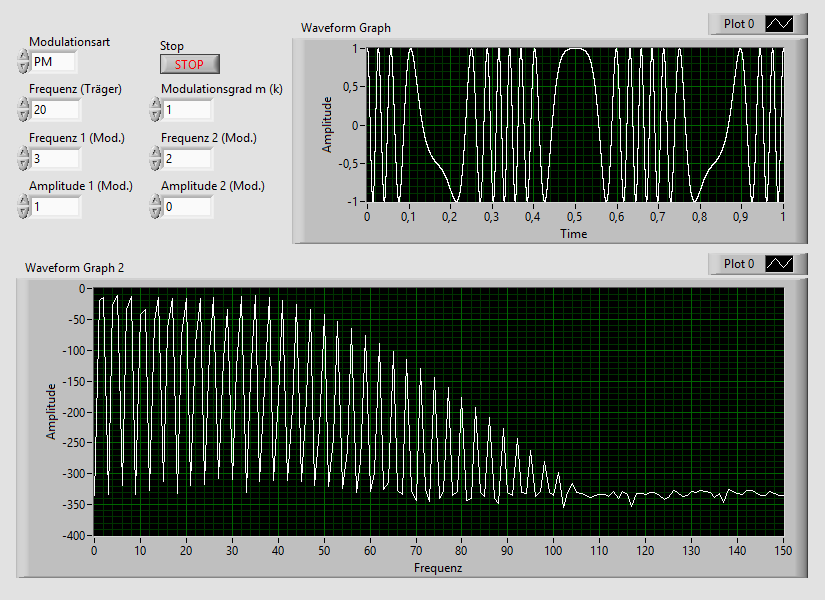
\includegraphics[width=0.9\textwidth]{pic/pm_example.png}
		\caption{Phasenmodulation}
		\label{fig:pm_example}	
	\end{subfigure}
	\caption{Frontpanel des Modulations-VIs bei frequenz- und phasenmoduliertem Signal.}
\end{figure} 

\pagestyle{headings}
Mit dem nun vollständigen Modulations-VI konnten nun auch Signale erzeugt werden, die von der Messstruktur nicht demoduliert werden können.
Die letzte Aufgabe war es die Messstruktur so zu vervollständigen, dass auch frequenz- und phasenmodulierte Signale demoduliert werden können.
Für diese letzte Erweiterung mussten nur zwei weitere Cases eingebaut werden.
Durch ableiten des Signals, wird das zu modulierende Signal ein Teil der Amplitude, weswegen die beiden anderen Modulationstypen mit den gleichen Verfahren demoduliert werden können wie bei der AM.
Abbildung \ref{fig:messstruktur_dafpm} stellt das vollständige Messstruktur-VI dar.
Dieses unterscheidet sich von der Abbildung \ref{fig:messstruktur_dam} nur in den zwei weiteren Cases, der Erweiterung der Speicherfunktion um die Amplituden in den Zeitbildern nach Demodulation/Tiefpass bzw. Bandpass, welcher den Tiefpass ersetzt um ebenfalls den Gleichanteil zu filtern.
	
\

Der erste Case liegt vor der Demodulationsoperation und ist für FM und PM gleich.
Hier wird nur das Signal über ein Express-VI abgeleitet und nach der Konvertierung in diesem VI wieder in eine Waveform zurück konvertiert.
Im Falle der AM geschieht nichts in dem Case, die Kabel gehen also einfach durch diesen durch.
Da nach dem Ableiten bei dem frequenzmodulierten Signal $S_\text{FM}(t)$ das zu modulierende Signal $S(t)$ nun in der Amplitude steht, kann dieses wie ein amplitudenmoduliertes Signal behandelt werden.
	
\

In dem zweiten neuen Case geschieht im Falle der AM und FM also nichts, auch hier verlaufen die Kabel direkt durch den Case.
Bei einem phasenmodulierten Signal befindet sich jedoch nicht das zu modulierende Signal $S(t)$, sondern dessen Ableitung in der Amplitude, weswegen der zweite Case hier genutzt wird, um das Signal einmal zu integrieren, analog zu der Differentiation in dem ersten Case.
Das Frontpanel für ein Beispielsignal ist in Abb. \ref{fig:dpm} dargestellt. 
Wie auch bei den anderen Beispielen sind weitere im Anhang (Abschnitt \ref{sec:anhang}) vorzufinden.

\newpage
\pagestyle{empty}
\begin{figure}[H]
	\centering
	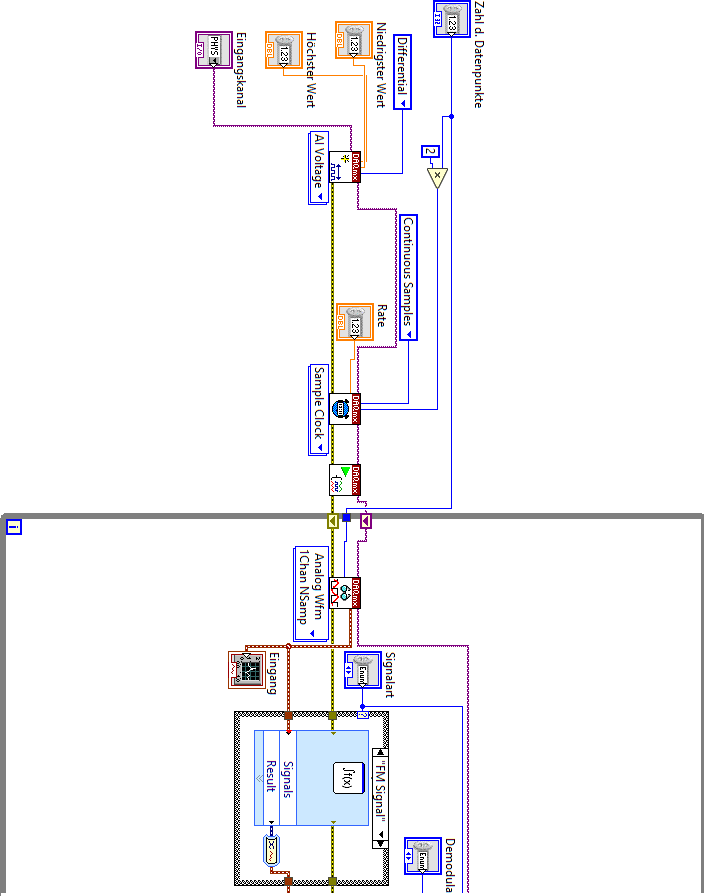
\includegraphics[width=\textwidth]{pic/messstruktur_dafpm1.png}
\end{figure} 
\begin{figure}[H]
	\centering
	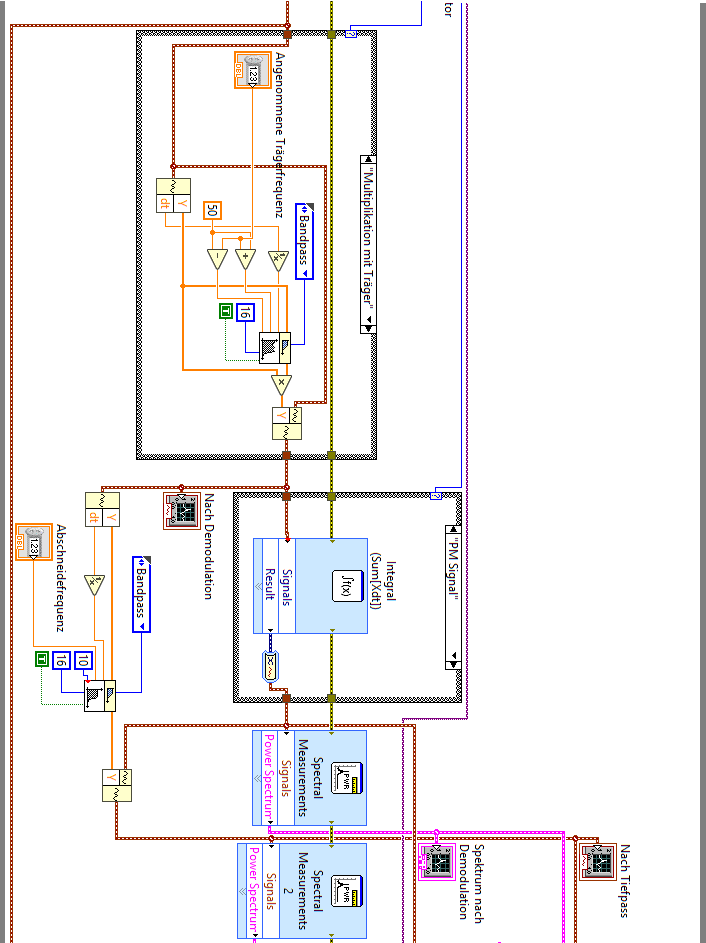
\includegraphics[width=\textwidth]{pic/messstruktur_dafpm2.png}
\end{figure} 
\begin{figure}[H]
	\centering
	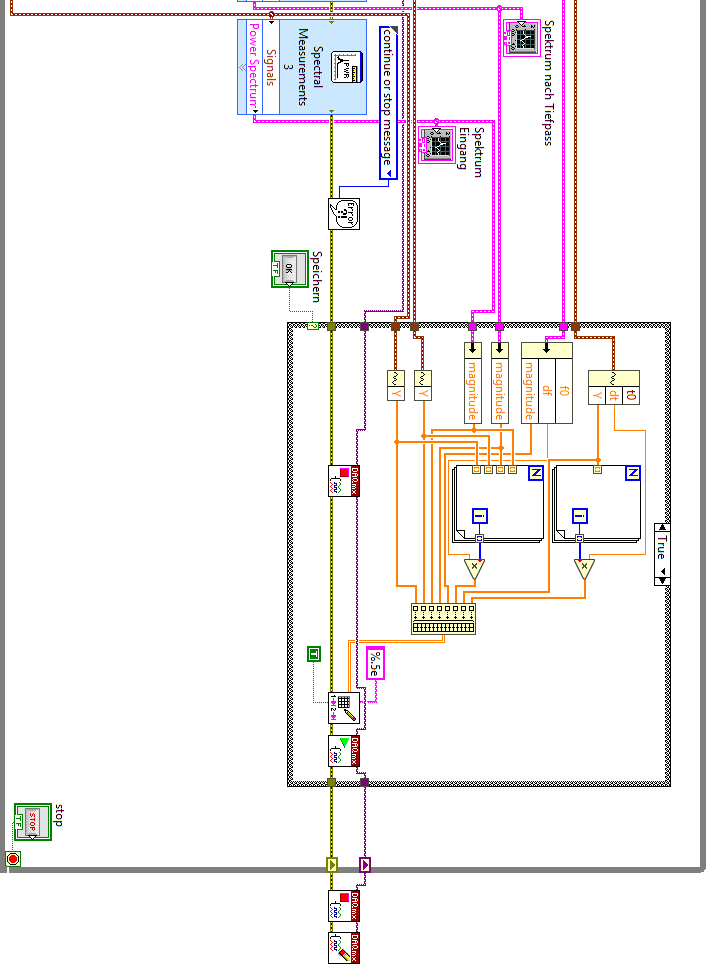
\includegraphics[width=\textwidth]{pic/messstruktur_dafpm3.png}
	\caption{LabVIEW VI der vollständigen Messstruktur mit Demodulationsoptionen für AM, FM und PM, sowie Speicherfunktion.}
	\label{fig:messstruktur_dafpm}	
\end{figure} 

\begin{figure}[H]
	\centering
	\begin{subfigure}[c]{\textwidth}
		\centering
		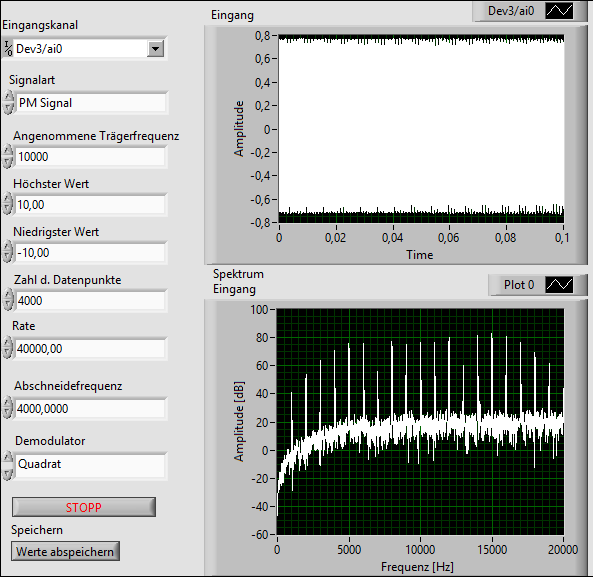
\includegraphics[width=0.7\textwidth]{pic/dpm1.png}
		\subcaption{Linke Seite des Frontpanels mit Parametern und Graphen für das Eingangssignal.}
	\end{subfigure}
	\begin{subfigure}[c]{\textwidth}
		\centering
		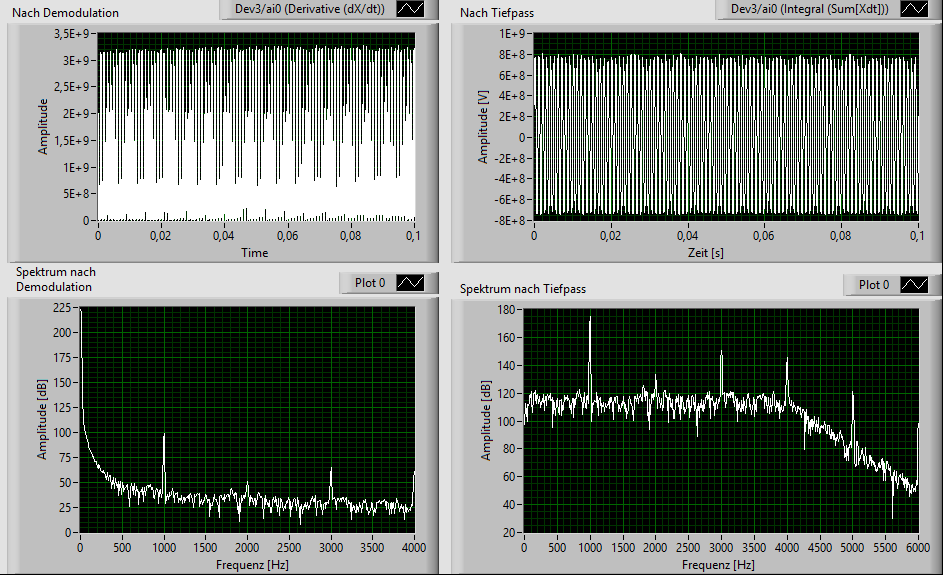
\includegraphics[width=0.9\textwidth]{pic/dpm2.png}
		\subcaption{Rechte Seite des Frontpanels mit Graphen für das demodulierte Signal vor und nach Bandpass.}
	\end{subfigure}	
	\caption{Frontpanel der vollständigen Messstruktur bei eingehendem PM-Signal von dem Modulations-VI.}
	\label{fig:dpm}	
\end{figure} 
\pagestyle{headings}